\section{The Integration Algorithm}

The purpose of performing an intensity integration is 
to create a plot of average intensity as a function
of either $Q$, $2\theta$, or $\chi$. The algorithm
for performing an intensity integration is pretty
straight foreward. In order to perform an intensity
integration, we must already know the calibration values
of the experiment for the paritcular image that will
be integrated. Than, a range and bin size for the
integration must be give. For example, you might
want to do a $Q-I$ integration from 2 to 5 with
100 bins. Whatever the range is, it 
must be specified before an integration is done.

The algorithm for performing the intensity integration
is as follows: loop over every pixel in the image. 
Add its intensity to the bin if it should be
in the bin based upon its value of $Q$, $2\theta$, or 
$\chi$. Remember that we need to use the calibration
values to calculate the correspondign $Q$, $2\theta$, and 
$\chi$ value using equation~\ref{ytermsydoubleprime}
\ref{xtermsxdoubleprime}, \ref{chitermsyx}, 
\ref{2thetatermsr}, and \ref{qterms2theta}.
After going through all the pixel, the bins then get averaged 
together. 

This program can constran the integration. 
This means that you can perform, for example,
a $Q$ integration of only those pixels with some
particular range of $\chi$ values. Or, you can
constaint your $\chi$ integration to on a particular
$Q$ range. This could be used, for example, to
perform a $\chi$ integration of only a particular
diffraction peak. The algorithm for performing
the constaint isn't any more complicated. You just
only bin a particular intensity value if it is
allowed by the constraint.

The program can allows for masking of pixels.
This complicates the algorithm a little bit further.
Whenever the program finds an intensity value
that should be masked (either because it is too 
large, too small, or in a polygon mask), it makes
sure not to bin that pixel and acts as though
it does not exist..

Finally, the program can perform a polarization 
correction to the integration. The polarization 
correction formula is
\begin{align}
    I&=Im/PF \\ 
    PF&=P(1 - (\sin(2\theta)\sin(\chi-90))^2) + 
    (1 - P)(1 - (\sin(2\theta)\cos(\chi-90))^2)
\end{align}
with $Im$ the measured intensity. If this
is selected, what happens
then is that all pixels have their intensity
value corrected by this formula before they
are binned. Note that the $2\theta$ and $\chi$
values correspond to the particular value
that is being corrected.

\section{Integrating with the Program}


In order to perform a cake of the program you will have to 
already have loaded into the program one or more diffraction
data files and you will ahve to input calibraiton data
into the program. Figure~\ref{integration_page} shows the
\gui{Integrate} tab. This is where integration is done.
Notice that there are two seperate inputs on the page. 
The input on the left is titled \gui{Q-I Integration}
and is for performign $Q$ integration.
The inputs on the left allow you to specify a
range in $Q$ that should be integrated.
The $Q$ range can be inputted with the
\gui{Q Lower?}, \gui{Q Upper?} inputs. The number of
bins in $Q$ space can be specified with the
\gui{Number of Q?} input. 
To perform a $Q$ integration, you have to push
the \gui{Integrate} button on the left.

\begin{SCfigure}[1][htb]
\centering
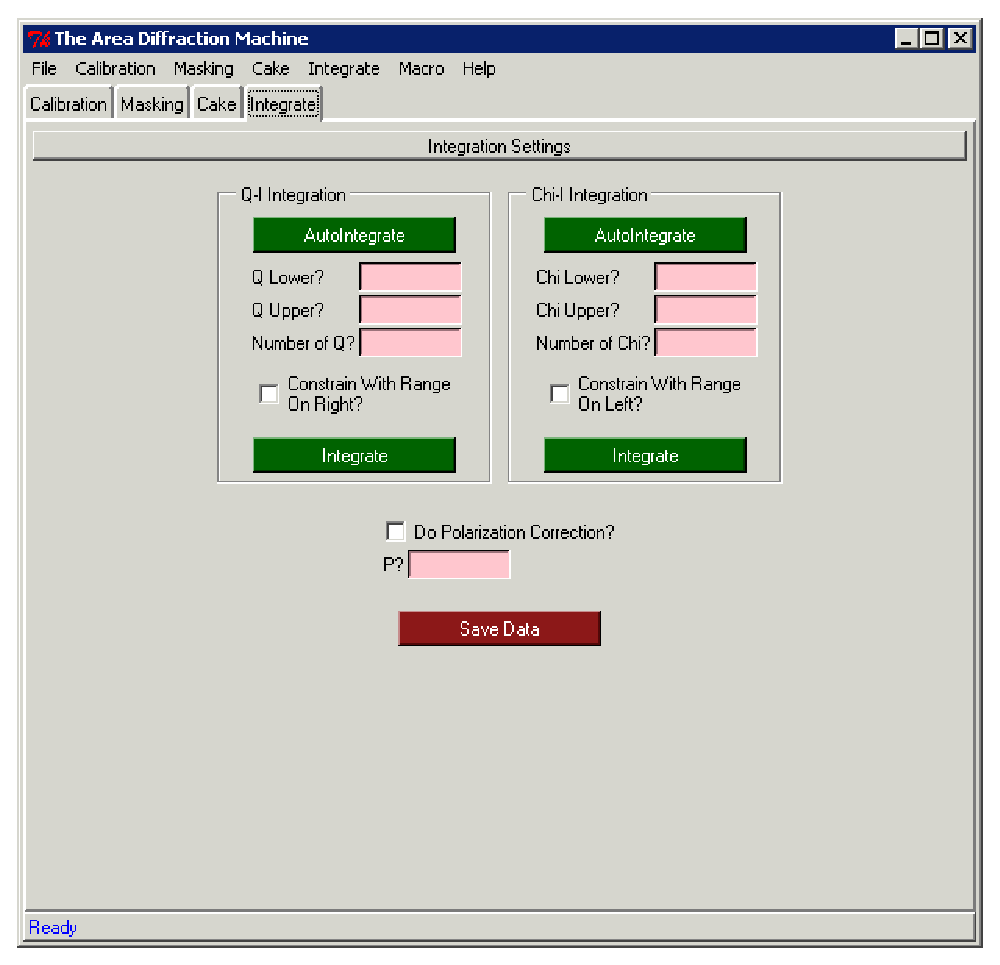
\includegraphics[scale=.75]{figures/integration_page.eps}
\caption{A screen shot of the integration tab to the 
    program. This is the tab where you can integrate data.} 
\label{integration_page}
\end{SCfigure}

To perform a $\chi$ integration, you can use the inputs
on the right under the name \gui{Chi-I Integration}.
The inputs on the right allow you to spccify
a rnage in $\chi$ with the \gui{Chi Lower?} and
\gui{Chi Upper?} inputs. The number of bins in
$\chi$ space can be specified with the
\gui{Number of Chi?} input. To perform the
$\chi$ integraiton, you ahve to push the
\gui{Integrate} button on the right.

\subsection{The Integration Window}

\begin{SCfigure}[1][htb]
\centering
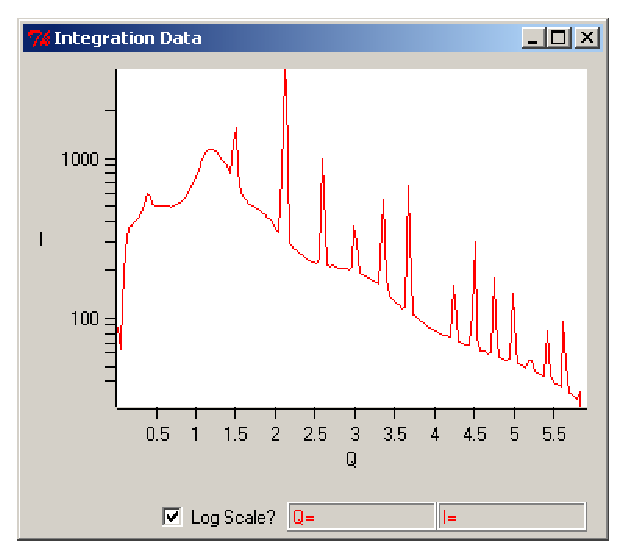
\includegraphics[scale=.75]{figures/integration_window_q.eps}
\caption{A screen shot of the integration window that
    opens up after you perform an intensity integration.} 
\label{integration_window_q}
\end{SCfigure}

\begin{SCfigure}[1][htb]
\centering
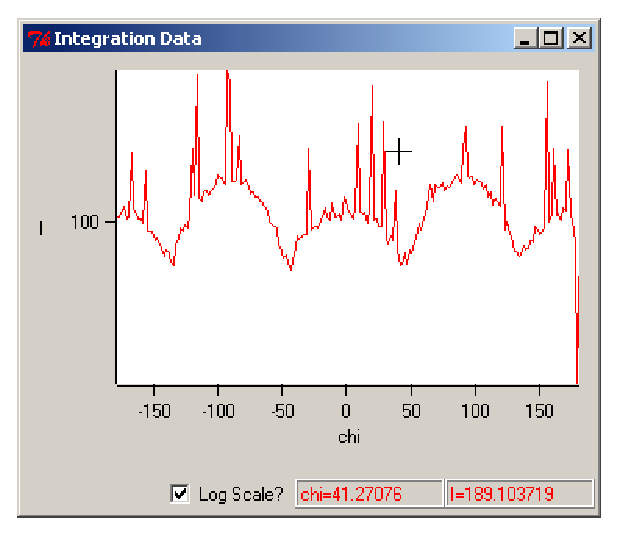
\includegraphics[scale=.75]{figures/integration_window_chi.eps}
\caption{A screen shot of the integration window that
    opens up after you perform an intensity integration.} 
\label{integration_window_chi}
\end{SCfigure}

After you push the integrate button, a line plot of the 
integrated data will be displayed in a new window. 
Figure~\ref{integration_window_q} shows 
the window displaying $Q$ integrated data
and figure~\ref{integration_window_chi} shows the
window displaying $\chi$ integrated ata.
Similar to the diffraction data display and the cake 
data display, this window has a couple of nice featuers
\begin{itemize}
    \item {\em Zoom into the data} - To zoom, left click
    on the data and hold down on the mouse. When you drag 
    the cursor, the program will create a resizing square. 
    When you let go of the mouse, the selected square will 
    be used as the outer bound and the image will be zoomed 
    into it. 
    \item {\em Zoom out of the data} - To unzoom, right
    click on the graph
    \item {\em Resize the window} - This will make the graph
    either larger or smaller. To do so, click on the bottom 
    right corner and drag. 
    \item {\em Read coordinates for a selected point} -
    When you mouse over the graph, the selected $Q$ (or $\chi$
    or $2\theta$) and intensity value will be displayed.
    \item {\em Log Scaling} - The \gui{Log Scale?} checkbox
    will toggle wheter to display a log scale of the data.
\end{itemize}

\subsection{AutoIntegrate}


\subsection{Masking}
\subsection{Working in $2\theta$}
\subsection{Saving Integrated Data}




